\section{Introdução}
\label{sec:intro}



%\lipsum[1]

O ramo da visão computacional é bastante diverso e possui variadas aplicações. Para tais aplicações, frequentemente tem-se o problema de relacionar o cenário digital(as imagens bidimensionais obtidas por câmeras) com o cenário real% em que se é bastante familiarizado.

À medida com que uma pessoa cresce, adquire-se a capacidade de relacionar a imagem obtida pelos olhos com o seu significado real e isso é feito principalmente através de aprendizado: aprende-se o tamanho e forma dos objetos do dia a dia e através da inferência, por comparação pode-se ter uma estimativa de posicionamento de objetos bem como seu tamanho.

Já para câmeras digitais que se comportam de forma diferente ao olho humano na captura de imagens, existem incertezas relacionadas à câmera que se dividem em dois grupos:

\begin{description}
\item[Intrínseco] Inerentes ao processo de fabricação da câmera.%Tais como alinhamento
\item[Extrinseco] Relativos à posição da câmera em relação ao espaço.%Devido à posição da origem e orientação dos eixos. 
\end{description}

Por esse motivo, utiliza-se conceitos de algebra linear, geometria e ótica para relacionar o espaço da imagem obtida pela câmera com a posição real do ponto observado. Essa relação pode ser dada pela Equação (\ref{eq:matrizes}) utilizando-se coordenadas homogêneas, em que a matriz $In$ relaciona os parâmetros intrínsecos e a matriz $Ex$ relaciona os parâmetros extrinsecos. A Figura (\ref{fig:PinholeCamera}) mostra alguns dos parâmetros apresentados na Equação (\ref{eq:matrizes}).

\begin{equation}
\label{eq:matrizes}
s
\begin{bmatrix}
u \\
v \\
1
\end{bmatrix}
=
\underbrace{
\begin{bmatrix}
f_x & 0 & c_x \\
0 & f_y & c_y \\
0 & 0 & 1
\end{bmatrix}}_{In}
\underbrace{
\begin{bmatrix}
r_{11} & r_{12} & r_{13} & t_{1} \\
r_{21} & r_{22} & r_{23} & t_{2} \\
r_{31} & r_{32} & r_{33} & t_{3}
\end{bmatrix}}_{Ex}
\begin{bmatrix}
X \\
Y \\
Z \\
1
\end{bmatrix}
\end{equation} 

\begin{figure}[!ht]
\centering
\label{fig:PinholeCamera}
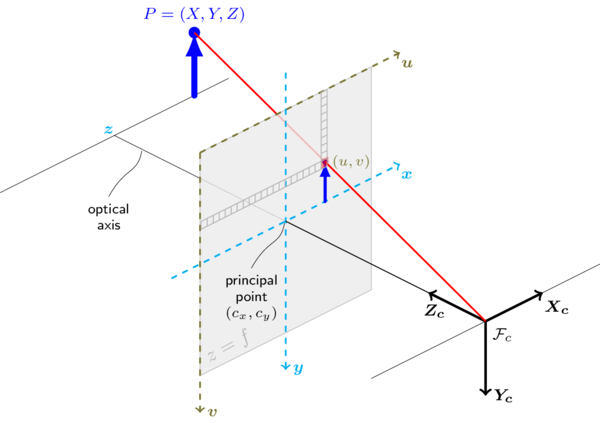
\includegraphics[width=0.3\textwidth]{img/PinholeCameraModel.png}
\caption{Modelo da câmera Pinhole}
\end{figure}

Segundo Fulano, é necessário apenas 6 pontos para determinar todos os parâmetros intrínsecos e extrínsecos da câmera. Mas para aumentar a precisão dos parâmetros e diminuir a incerteza associada, pode-se utilizar mais pontos conhecidos. % Explicar melhor sobre a determinação de pontos

Contudo, como toda a teoria exposta para calibração de câmera considera o modelo de câmera Pinhole e as câmeras digitais são feitas de diversas formas como mostra Raskar\cite{raskar}. Devido a essa variação entre câmeras, existem câmeras que autoajustam seu foco e portanto os parâmetros intrínsecos variam.